%% Beginning of file 'sample701.tex'
%%
%% Version 7.0.1. Created May 2025.
%% Version 7. Created January 2025.  
%%
%% AASTeX v7+ calls the following external packages:
%% times, hyperref, ifthen, hyphens, longtable, xcolor, 
%% bookmarks, array, rotating, ulem, and lineno 
%%
%% RevTeX is no longer used in AASTeX v7+.
%%
\documentclass[linenumbers,trackchanges,twocolumn]{aastex701}
%%
%% This initial command takes arguments that can be used to easily modify 
%% the output of the compiled manuscript. Any combination of arguments can be 
%% invoked like this:
%%
%% \documentclass[argument1,argument2,argument3,...]{aastex701}
%%
%% Six of the arguments are typestting options. They are:
%%
%%  twocolumn   : two text columns, 10 point font, single spaced article.
%%                This is the most compact and represent the final published
%%                derived PDF copy of the accepted manuscript from the publisher
%%  default     : one text column, 10 point font, single spaced (default).
%%  manuscript  : one text column, 12 point font, double spaced article.
%%  preprint    : one text column, 12 point font, single spaced article.  
%%  preprint2   : two text columns, 12 point font, single spaced article.
%%  modern      : a stylish, single text column, 12 point font, article with
%% 		  wider left and right margins. This uses the Daniel
%% 		  Foreman-Mackey and David Hogg design.
%%
%% Note that you can submit to the AAS Journals in any of these 6 styles.
%%
%% There are other optional arguments one can invoke to allow other stylistic
%% actions. The available options are:
%%
%%   astrosymb    : Loads Astrosymb font and define \astrocommands. 
%%   tighten      : Makes baselineskip slightly smaller, only works with 
%%                  the twocolumn substyle.
%%   times        : uses times font instead of the default.
%%   linenumbers  : turn on linenumbering. Note this is mandatory for AAS
%%                  Journal submissions and revisions.
%%   trackchanges : Shows added text in bold.
%%   longauthor   : Do not use the more compressed footnote style (default) for 
%%                  the author/collaboration/affiliations. Instead print all
%%                  affiliation information after each name. Creates a much 
%%                  longer author list but may be desirable for short 
%%                  author papers.
%% twocolappendix : make 2 column appendix.
%%   anonymous    : Do not show the authors, affiliations, acknowledgments,
%%                  and author contributions for dual anonymous review.
%%  resetfootnote : Reset footnotes to 1 in the body of the manuscript.
%%                  Useful when there are a lot of authors and affiliations
%%		    in the front matter.
%%   longbib      : Print article titles in the references. This option
%% 		    is mandatory for PSJ manuscripts.
%%
%% Since v6, AASTeX has included \hyperref support. While we have built in 
%% specific %% defaults into the classfile you can manually override them 
%% with the \hypersetup command. For example,
%%
%% \hypersetup{linkcolor=red,citecolor=green,filecolor=cyan,urlcolor=magenta}
%%
%% will change the color of the internal links to red, the links to the
%% bibliography to green, the file links to cyan, and the external links to
%% magenta. Additional information on \hyperref options can be found here:
%% https://www.tug.org/applications/hyperref/manual.html#x1-40003
%%
%% The "bookmarks" has been changed to "true" in hyperref
%% to improve the accessibility of the compiled pdf file.
%%
%% If you want to create your own macros, you can do so
%% using \newcommand. Your macros should appear before
%% the \begin{document} command.
%%
\newcommand{\vdag}{(v)^\dagger}
\newcommand\aastex{AAS\TeX}
\newcommand\latex{La\TeX}

\newcommand{\Mdot}{\mathrm{M}_{\odot}}
\newcommand{\Rdot}{\mathrm{R}_{\odot}}
\newcommand{\Ldot}{\mathrm{L}_{\odot}}
\newcommand{\Myr}{\mathrm{Myr}}
\newcommand{\red}{\textcolor{red}}
%%%%%%%%%%%%%%%%%%%%%%%%%%%%%%%%%%%%%%%%%%%%%%%%%%%%%%%%%%%%%%%%%%%%%%%%%%%%%%%%
%%
%% The following section outlines numerous optional output that
%% can be displayed in the front matter or as running meta-data.
%%
%% Running header information. A short title on odd pages and 
%% short author list on even pages. Note that this
%% information may be modified in production.
%%\shorttitle{AASTeX v7.0.1 Sample article}
%%\shortauthors{The Terra Mater collaboration}
%%
%% Include dates for submitted, revised, and accepted.
%%\received{February 1, 2025}
%%\revised{March 1, 2025}
%%\accepted{\today}
%%
%% Indicate AAS Journal the manuscript was submitted to.
%%\submitjournal{PSJ}
%% Note that this command adds "Submitted to " the argument.
%%
%% You can add a light gray and diagonal water-mark to the first page 
%% with this command:
%% \watermark{text}
%% where "text", e.g. DRAFT, is the text to appear.  If the text is 
%% long you can control the water-mark size with:
%% \setwatermarkfontsize{dimension}
%% where dimension is any recognized LaTeX dimension, e.g. pt, in, etc.
%%%%%%%%%%%%%%%%%%%%%%%%%%%%%%%%%%%%%%%%%%%%%%%%%%%%%%%%%%%%%%%%%%%%%%%%%%%%%%%%
%%
%% Use this command to indicate a subdirectory where figures are located.
%%\graphicspath{{./}{figures/}}
%% This is the end of the preamble.  Indicate the beginning of the
%% manuscript itself with \begin{document}.

\begin{document}

\title{Weird stuff from not so weird stuff}%\footnote{Footnotes can be added to titles}}

%% A significant change from AASTeX v6+ is in the author blocks. Now an email
%% address is required for each author. This means that each author requires
%% at least one of the following:
%%
%% \author
%% \affiliation
%% \email
%%
%% If these three commands are not available for each author, the latex
%% compiler will issue an error and if you force the latex compiler to continue,
%% it will generate an incomplete pdf.
%%
%% Multiple \affiliation commands are allowed and authors can also include
%% an optional \altaffiliation to indicate a status, i.e. Hubble Fellow. 
%% while affiliations are indexed as footnotes, altaffiliations are noted with
%% with a non-numeric footnote that is set away from the numeric \affiliation 
%% footnotes. NOTE that if an \altaffiliation command is used it must 
%% come BEFORE the \affiliation call, right after the \author command, in 
%% order to place the footnotes in the proper location. Because non-numeric
%% symbols are used, \altaffiliation should be used sparingly.
%%
%% In v7+ the \author command takes an optional argument which provides 
%% additional metadata about the author. Authors can provide the 16 digit 
%% ORCID, the surname (family or last) name, the given (first or fore-) name, 
%% and a name suffix, e.g. "Jr.". The syntax is:
%%
%% \author[orcid=0000-0002-9072-1121,gname=Gregory,sname=Schwarz]{Greg Schwarz}
%%
%% This name metadata in not shown, it is only for parsing by the peer review
%% system so authors can be more easily identified. This name information will
%% also be sent to the publisher so they can include it in the CROSSREF 
%% metadata. Including an orcid will hyperlink the author name to the 
%% author's ORCID page. Note that  during compilation, LaTeX will do some 
%% limited checking of the format of the ID to make sure it is valid. If 
%% the "orcid-ID.png" image file is  present or in the LaTeX pathway, the 
%% ORCID icon will appear next to the authors name.
%%
%% Even though emails are now required for each author, the \email does not
%% produce output in the compiled manuscript unless the optional "show" command
%% is used. For example,
%%
%% \email[show]{greg.schwarz@aas.org}
%%
%% All "shown" emails are show in the bottom left of the first page. Due to
%% space constraints, only a few emails should be shown. 
%%
%% To identify a corresponding author, use the \correspondingauthor command.
%% The command appends "Corresponding Author: " to the argument it appears at
%% the bottom left of the first page like the output from \email. 

\author[orcid=0000-0000-0000-0001,sname='North America']{Neev Shah}
\affiliation{Steward Observatory, The University of Arizona}
\email[show]{neevshah@arizona.edu}  

% \author[orcid=0000-0000-0000-0002,gname=Bosque, sname='Sur America']{Mathieu Renzo} 
% \affiliation{Steward Observatory, The University of Arizona}
% \email{mrenzo@arizona.edu}

% \author[orcid=0000-0000-0000-0002,gname=Bosque, sname='Sur America']{Koushik Sen} 
% \affiliation{Steward Observatory, The University of Arizona}
% \email{ksen@arizona.edu}

% \author[orcid=0000-0000-0000-0002,gname=Bosque, sname='Sur America']{Aldana Grichener} 
% \affiliation{Steward Observatory, The University of Arizona}
% \email{agrichener@arizona.edu}

%% Use the \collaboration command to identify collaborations. This command
%% takes an optional argument that is either a number or the word "all"
%% which tells the compiler how many of the authors above the command to
%% show. For example "\collaboration[all]{(DELVE Collaboration)}" wil include
%% all the authors above this command.
%%
%% Mark off the abstract in the ``abstract'' environment. 
\begin{abstract}

\red{TBA}

\end{abstract}

%% Keywords should appear after the \end{abstract} command. 
%% The AAS Journals now uses Unified Astronomy Thesaurus (UAT) concepts:
%% https://astrothesaurus.org
%% You will be asked to selected these concepts during the submission process
%% but this old "keyword" functionality is maintained in case authors want
%% to include these concepts in their preprints.
%%
%% You can use the \uat command to link your UAT concepts back its source.
\keywords{\red{TBA}}%\uat{Galaxies}{573} --- \uat{Cosmology}{343} --- \uat{High Energy astrophysics}{739} --- \uat{Interstellar medium}{847} --- \uat{Stellar astronomy}{1583} --- \uat{Solar physics}{1476}}

%% From the front matter, we move on to the body of the paper.
%% Sections are demarcated by \section and \subsection, respectively.
%% Observe the use of the LaTeX \label
%% command after the \subsection to give a symbolic KEY to the
%% subsection for cross-referencing in a \ref command.
%% You can use LaTeX's \ref and \label commands to keep track of
%% cross-references to sections, equations, tables, and figures.
%% That way, if you change the order of any elements, LaTeX will
%% automatically renumber them.

\section{Introduction}
\red{
\begin{enumerate}
    \item Background
    \item Introduce XRBs, runaways, HMXBs - 4U1700-37 - well studied, many observational constraints - not well known if NS or not
    \item Introduce GWs  - GW190814 - unknown origin, conventionally difficult to form
    \item Lower mass gap - GW190814, new NSBH GW, some EM observations in the mass gap as well. Unknown if real or not
    \item Connection between XRBs and GWs - XRBs perhaps intermediate path.
    \item Leverage XRB constraints to chart past history, connect it to GW190814 at low Z
    \item What exactly are we trying to show? Forming asymmetric mass ratio systems starting from symmetric, followed by conservative mass transfer. Kick can lead to variety of outcomes, including XRBs, TZOs, GWs. GW190814 not a weirdo to be ignored
    \item Why is it important
    \item Describe paper outline
\end{enumerate}
}

Massive stars ($> 8-10\,\Mdot$) end their lives in energetic explosions or implosions, leaving behind a compact object remnant like a black hole (BH) or a neutron star (NS). Since most massive stars live in binaries and higher order systems \cite{2012Sci...337..444S,2023ASPC..534..275O}, they are likely to interact at some point in their short lifetimes. Such systems are thought to be the progenitors of a wide range of high energy phenomena, such as X-ray binaries (XRB), stripped envelope supernovae, gravitational wave (GW) sources \cite{2023PhRvX..13d1039A}, gamma--ray bursts (GRB), and various other transients. The formation of such systems is directly affected by the uncertainties in our understanding of massive stars, such as the wind mass loss rates in various phases of evolution, impact of rotation and other mixing processes, and their explodability which determines whether they form NS's, direct collapse BH's, or fallback BH's. These in turn couple with the uncertainties in binary evolution such as the stability and conservativeness of mass transfer (MT), common envelope (CE) evolution, and the transport of matter and angular momentum from one star to its companion. 

Among the many rare and common outcomes of binary evolution, XRBs and GW events provide a unique insight to the end stages of massive binaries. These systems require the presence of a compact object in the binary, which implies that the progenitor system consisted of at least one massive star that has reached the end of its life. While XRBs have been observationally studied in the Milky Way and nearby galaxy for decades, the direct detection of GWs from compact object mergers in 2015 has reignited interest in understanding these rare products of massive binary evolution. For compact binaries originating from the isolated binary channel, an XRB phase is also a necessary intermediate path, and provides a complementary insight to their formation. In the local universe, XRBs can be well studied and allow for an accurate measurement of component masses and various other properties of the binary orbit and the visible star. Since an XRB necessarily requires the binary to be bound after the first SN (or implosion), their rates also sensitively depend on the strength of the natal kicks received to the compact objects at the time of explosion (implosion). Such natal kicks often unbind the binary, ejecting the compact object and its companion in different directions. However, if the binary remains bound, it can also gain a systemic velocity depending on the mass lost at the time of SN and strength and direction of the natal kick. Most high--mass XRBs (HMXB) are indeed seen to be runaway systems, where they are observed to be moving faster than the local ISM from their place of origin, which sometimes is a young or open cluster. If the visible star in the XRB also has kinematic constraints, such as its proper motion and radial velocities, one can accurately trace the binary in time to find its birth cluster. If such an exercise is successful, this can give us estimate of the time of SN in the binary (kinematic age), under the hypothesis that the system got ejected from its birthplace when one of the stars in the binary ended its life in an explosion. The systemic velocity can also constraint the amount of mass lost in the explosion, which sets the pre-SN mass of the star that exploded. If one is also able to estimate the age of the birth cluster, through isochrone fitting for example, we can obtain a lower limit to the initial mass of the star that exploded. These observational constraints can help chart a pathway to recreating the past evolutionary history of the system, and provide a unique opportunity to test our models of massive binary evolution.  

The prototypical system for such a scenario is the HMXB 4U1700-37/ HD 153919. One of the first X--ray sources discovered in the 1970s, it consists of an O6.5 Iaf+ star, which is one of the most massive stars in known XRBs with an estimated mass of $40-60\,\Mdot$. The compact object in this system is equally interesting, with an estimated mass of $2.5\,\Mdot$, straddling the "mass--gap" between the heaviest neutron stars and lightest black holes. With the help of Gaia EDR3, and verified by \cite{2022MNRAS.511.4123H} using Gaia DR3, \cite{2021A&A...655A..31V} confirmed that this system originated from the young open cluster NGC 6231, and was ejected from it $\approx 2\,\Myr$ ago. Together with the young age of the NGC 6231 (few $\Myr$), this implies that the star that exploded had an initial mass $>\,30\,\Mdot$. The short period of the binary ($3.41$ days), highly asymmetric mass ratio, and age constraints have been challenging to interpret given our standard understand of binary evolution. \cite{2021A&A...655A..31V} proposed the system to have formed from a pair of massive stars that underwent mass transfer (MT) while the more massive (donor) star was stil on the Main Sequence (MS), termed as Case A MT. Given the short period of the binary today, they also hypothesized that the compact remnant received a natal kick in a favorable direction that shrank the orbit. The presence of a compact object in the mass--gap, and the highly asymmetric mass ratio of this system is particularly interesting, as it is very similar to GW190814, which also consisted of a merger between a compact object in the \textit{"lower mass gap"} and a $23\,\Mdot$ BH \cite{2020ApJ...896L..44A}. This event is also the most asymmetric merger seen in the first three observing runs of LIGO-Virgo-KAGRA (LVK), and has been challenging to interpret for most formation channels. Various explanations have been invoked for the formation of GW190814, such as a triple scenario requiring the merging of two NS's for creating a $2.5\,\Mdot$ compact object \cite{2021MNRAS.500.1817L}. Due to the mass segration in clusters, it is difficult to pair up compact objects of such unequal masses through dynamical interactions. While it may be possible to form such compact binaries through the isolated formation channel, this has been largely unexplored for the case of GW190814. Due to the unknown nature BH or NS nature of the lower mass compact object, it is also often categorized as an outlier to the BBH population. However, these results sensitively depend on the assumed parametric models for the mass distributions, and including or excluding it can significantly bias the minimum BH mass as measured on a population level \cite{2025arXiv250814159C,2021ApJ...913L...7A,2022ApJ...926...34E,2022ApJ...931..108F}. 

Our goal in this work is two--fold. We first utilize the rich set of observational constraints for the HMXB 4U1700-27/ HD 153919 (henceforth XRB) to estimate the properties of the binaries just prior to the first (and only) SN in the system. With the help of these constraints, we construct detailed binary evolution models computed with MESA to chart its past evolutionary history and likely progenitor system. In doing so, we demonstrate that forming this XRB through Case A MT is viable, as proposed originally in \cite{2021A&A...655A..31V}. We also show that a similar formation pathway can also work at lower metallicity, and lead to compact binaries with masses similar to what is seen in GW190814. We emphasize that our progenitor systems for explaining both the XRB and GW190814 are \textit{"fairly normal"}, and the strength and direction of natal kicks received at the time of first SN are crucial in determining the final fate of the system.

In Section (Methods), we describe our setup for computing the evolution of a binary system with MESA. We also describe our monte carlo method, wherein we use the observational constraints of a post-supernova binary to infer its properties pre-supernova. In Section (XRB), we demonstrate our monte carlo method by applying it to the HMXB, and constrain its pre-supernova properties. Motivated by those results, we use MESA to construct an evolutionary pathway for this system starting from a massive binary. We end the section with a discussion on the future evolution of the XRB, and its connection to TZO's. In Section (GW190814), we construct similar MESA models at lower metallicity to explore the formation of a GW190814-like system. We discuss the conditions in which such a system can form, and its similarities and differences with the HMXB described in the previous section. We also make toy estimates for the rates of such events, and what makes them rare. In Section (Conclusion), we summarize our results and discuss the implications of our work.

\section{Methods} \label{sec:methods}

\subsection{\texttt{MESA}}

We simulate the evolution of massive binaries using \texttt{MESA (r24.08.01)} \cite{2011ApJS..192....3P,2013ApJS..208....4P,2015ApJS..220...15P,2018ApJS..234...34P,2019ApJS..243...10P,2023ApJS..265...15J}. Our inlists and choice of input parameters are public (\red{link zenodo/github}) and we mention some of the relevant parameters and assumptions below.

\red{
\begin{enumerate}
    \item MESA (star) - basic stellar physics assumptions - MLT, overshooting, other mixing, rotation, winds, supereddington treatment
    \item MESA (binary) - Two stars evolved self consistently, along with orbit equations. Treatment of mass transfer (Kolb \& Ritter), AM transport, loss from system, tides, rotationally enhanced winds. Rotation only included in accretor, turned off in donor - justify why? 
    \item Monte Carlo - Outcome of supernova in a binary - Assumptions: Pre-SN circular orbits, instantaneous mass loss, Blauuw kick, Natal kick. Mass loss and kick vector gives post-SN orbital parameters, systemic velocity and eccentricity.
\end{enumerate}
}

We use the Ledoux criterion \cite{1947ApJ...105..305L} to find convective zones, and assume a mixing length parameter of 2.0. We also include semiconvection ($\alpha_{\mathrm{sc}}=1$) \cite{1983A&A...126..207L}, and thermohaline mixing ($\alpha_{\mathrm{th}}=1$) \cite{1980A&A....91..175K}. To account for convective boundary overshooting above the core, we use the exponentional model with free parameters $(f,f_0) = (4.25 \times 10^{-2}, 10^{-3})$, which broadly reproduces the width of the Main Sequence (MS) for a single $16 \, \Mdot$ star \cite{2011A&A...530A.115B}. We do not account for convective boundary over/undershooting for off-center convective layers. To aid in regions at the Eddington limit where convection is also inefficient, we utilize the local implicit enhancement of the convective flux in superadiabatic regions (\texttt{use superad reduction = .true.}) \cite{2023ApJS..265...15J}.

We only include rotation in our accretor models, while we fix the donor to be non--rotation (\red{explain why}). We treat rotation in the "shellular" approximation \cite{1992A&A...265..115Z,2012A&A...537A.146E}, where the angular velocities $\omega$ are fixed on isobaric surfaces (which requires strong anisotropic horizontal turbulence). We start our accretor models with a $\Omega/\Omega_{\mathrm{crit}} = 0$ at Zero--Age Main Sequence (ZAMS), but tidal effects tend to synchronize the star with the orbital period. \red{We also assume rigid rotation at the beginning of our runs at Zero--Age Main Sequence (ZAMS)}. We include several rotational mixing processes in a diffusion approximation, such as Eddington--Sweet circulation \cite{1950MNRAS.110..548S}, secular and dynamic shear instabilities, and the Goldreich-Schubert-Fricke (GSF) instability (see \cite{2000ApJ...528..368H} for a review of these processes). We assume a Spruit--Taylor dynamo \cite{2002A&A...381..923S} for treating the transport of angular momentum, and choose the same parameters as in \cite{2000ApJ...528..368H}. We also include the rotational enhancement of the wind mass loss \cite{1998A&A...329..551L} to keep the star to rotate sub--critically.  \red{We turn off rotation in the donor to avoid numerical issues, and because the spin of the compact object is largely unconstrainted for our XRB. Meanwhile, the companion is a visible star with a $vsin(i)$ measurement, and hence we do not ignore rotation in the accretor star. We do not believe that the rotation of the donor star has a significant effect in the interpretation of our results.} 

We include stellar winds by combining several different mass loss prescriptions. For stars with a surface effective temperature $\mathrm{T_{eff}} > 11000\,\mathrm{K}$, we utilize the mass loss prescriptions from \cite{2023A&A...676A.109B}, unless the surface hydrogen mass fraction falls below $0.4$, in which case we use the optically thick Wolf--Rayet (WR) wind mass loss rates from \cite{2000A&A...360..227N}. For cooler stars with a $\mathrm{T_{eff}} < 10000\,\mathrm{K}$, we use the mass--loss rates from \cite{2024A&A...681A..17D}, and interpolate linearly between the hot and cool winds for the temperature ranges $10000-11000\,\mathrm{K}$.

We treat mass transfer in a binary using an implicit scheme described in \cite{1990A&A...236..385K}. We assume that mass transfer is fully conservative until the accretor reaches $\Omega/\Omega_{\mathrm{crit}} = 0.9$, after which the mass--transfer efficiency depends on the rotationally enhanced wind mass loss. We assume that the specific angular momentum and entropy of the transferred mass is equal to the corresponding values at the surface of the accretor, and the chemical composition is set by the stratification of the donor. The transferred mass that is not accreted leaves the binary system carrying with it the specific angular momentum of the orbital motion of the accretor \cite{1997A&A...327..620S,2017MNRAS.471.4256V}. We also include tidal effects \cite{1981A&A....99..126H}, which can have a significant influence on the evolution of close binaries.

\subsection{Monte Carlo}

The occurence of a SN in a binary can have a significant effect on the orbital properties of the binary. There can be diverse post--SN outcomes in a binary depending on the amount of mass lost in the explosion and the strength and direction of a natal kick that the compact remnant may receive. This can lead to several observational consequences such as binary disruption, and if it remains bound, a change in the orbital period, eccentricity and even a systemic velocity to the binary as a whole. With the help of observational constraints on the parameters of a post--SN binary, we can try to infer its pre--SN parameters. We follow the setup in \cite{2024OJAp....7E..38E}, which in turn uses \cite{1994astro.ph.12023B} for calculating the outcomes of a SN in a binary. These calculations implicitly assume that the mass lost in a SN explosion is instantaneously lost from the system.

We start with generating an initial population of pre--SN binaries. The mass of the progenitor star that will undergo a SN is denoted. by $m_1$, while its companion has a mass $m_2$. We denote the pre--SN orbital period as $P_{\mathrm{pre-SN}}$. We also assume that the pre--SN binary orbit is circular. \red{This is justified for our scenario, because we model short period binaries that undergo mass transfer, and hence tides are expected to have circularized the orbit.} The post--SN binary properties depend on the pre--SN binary properties described above, and the details of the SN explosion. The relevant parameters are the amount of mass lost in the SN ($\Delta m$), and the speed ($v_{\mathrm{kick}}$) and direction $\{\theta, \,\phi\}$ of the compact object natal kick. We also assume that the companion star does not change in mass during the SN. This specifies all the relevant parameters needed to generate the post--SN population from the pre--SN binary population. 

\begin{figure}[htbp]
    \centering
    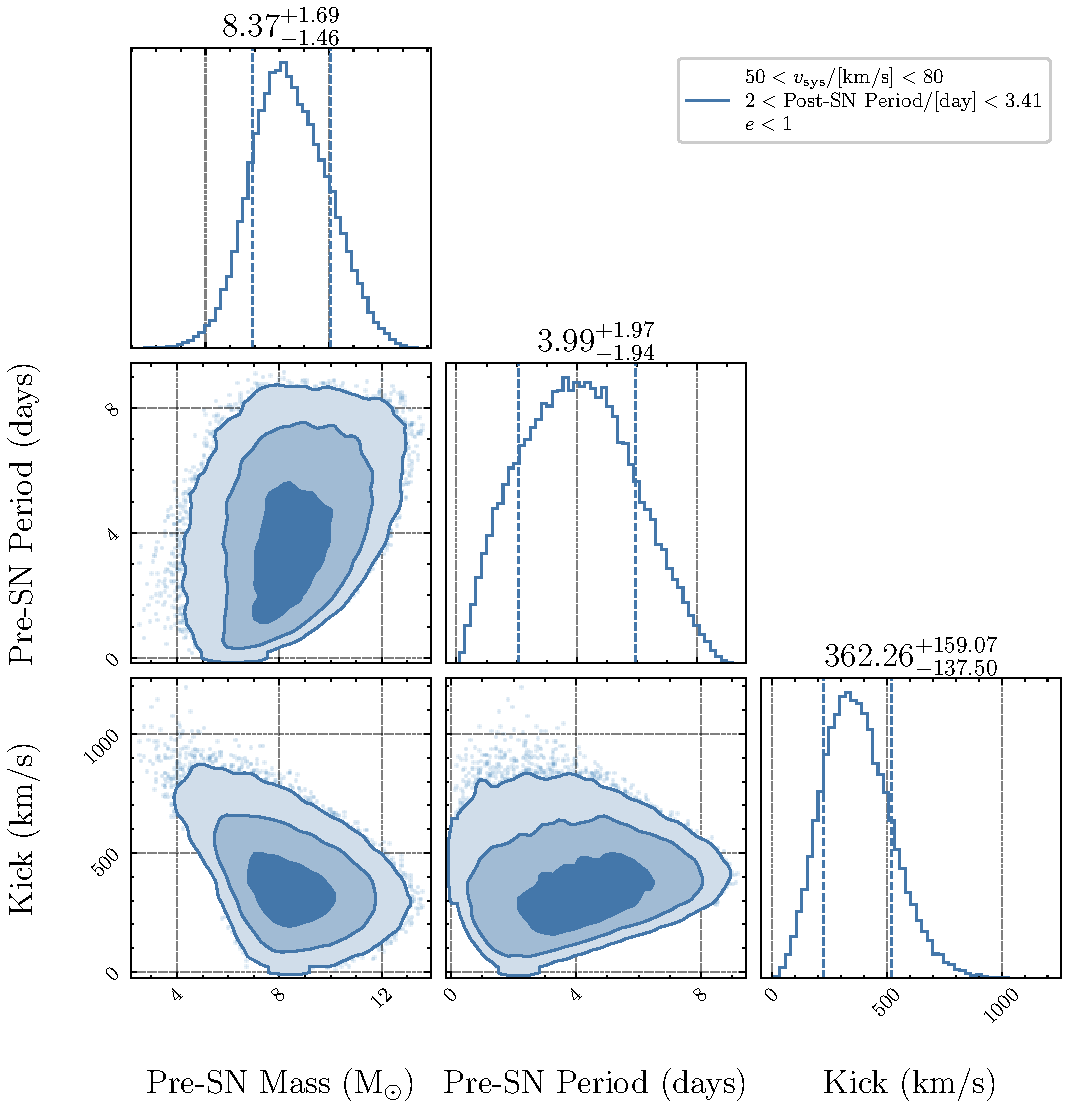
\includegraphics[width=0.5\textwidth]{xrb-monte-carlo-mass-period-kick.pdf}
    \caption{Corner plot showing the distributions of the pre--SN mass, pre--SN period and natal kick strength of the binary population that satisfy the observational constraints of the HMXB 4U1700-37/ HD 153919.}
    \label{fig:xrb_monte_carlo}
\end{figure}

\section{Results}

\subsection{Monte Carlo Results} \label{sec:monte_carlo}

\red{
\begin{enumerate}
    \item Describe what we are doing in this section - Infer pre-SN parameters of XRB from observational constraints
    \item Define relevant variables, initial population, assumptions (circular orbits) outcomes
    \item Emphasize that population is not observationally motivated, so probabilities arent real. Meant to explore parameter space
    \item Simulate outcomes of SN kicks - put observational constraints (define them)
    \item Show corner plot - explain what it implies - Pre-SN period and mass constraints
    \item Explain lower left corner gap in Pre-SN period - emphasize why kick is likely (based on MT period widening, Renzo+19), and kick needed to shrink
    \item Explain black shaded area - unlikely to fit without RLOF, theoretcially not expected due to orbit widening, wind mass loss over kinematic age gives minimum period ~2d. In black is shown distribution for post-SN period >~2d
\end{enumerate}
}

We use the monte carlo simulations described in Section \ref{sec:methods} to infer the pre--SN properties of the runaway HMXB 4U1700-37/ HD 153919. We utilize several of its observational constraints such as the masses of the companion star and the compact object, the current orbital period, and its systemic velocity with respect to its parent cluster NGC 6231. We generate a population of $10^7$ binaries with the mass of the companion star ($m_2$) sampled uniformly between $40-60\,\Mdot$. This roughly spans the estimated mass of the companion today, and we do not expect it to have significantly changed during the SN and the couple of $\mathrm{Myr}$ since then. We fix the post--SN mass of the compact object to be $2.5 \, \Mdot$, and sample the mass lost in the SN explosion ($\Delta m$) uniformly between $0-20 \, \Mdot$. This gives the pre--SN mass of the progenitor of the compact object as $m_1 = 2.5\, \Mdot + \Delta m$. We sample the pre--SN period of the binary uniformly between $0-30\, \mathrm{days}$. Although we allow for extremely short periods pre--SN, they are not realistic as the binaries are unlikely to fit inside a very small orbit. We sample the natal kicks to the compact object from a maxwellian distribution with a scale of $265 \, \mathrm{km/s}$. We have defined the pre--SN binary population ($m_1\,, m_2\,, P$) and the relevant parameters for the SN explosion ($\Delta m\,, v_{\mathrm{kick}}\,, \phi,\, \theta$) which allows us the compute the properties of the post--SN binary (or disrupted) population. From the post--SN population, we select for systems that are bound $e<1$ and have gained a systemic velocity between $50-80 \, \mathrm{km/s}$ \cite{2021A&A...655A..31V}. The present--day orbital period of the XRB is $3.41 \, \mathrm{days}$ \cite{2016MNRAS.461..816I}, but it is possible that the period immediately post--SN period was smaller and it has widened due to wind mass loss from the companion star since then. To account for this, we select for systems that have a post--SN orbital period between $2-3.41 \, \mathrm{days}$. We place a lower limit of $2 \, \mathrm{days}$, as smaller periods would imply that the companion star would have filled its Roche Lobe post--SN which does not seem plausible given the current evolutionary state of the star. 

\red{The systemic velocity inherited during the SN is 50-80km/s (the measured systemic velocity with respect to the open cluster is ~65km/s). Here, we are making the assumption that most of the systemic velocity of the XRB with respect to its birth cluster today can be attributed to its post--SN systemic velocity. We are also implicitly assuming that this velocity has not significantly changed during its runaway phase for the past couple of Myr. However, the details of this would depend on accurately modeling the effects of the cluster potential, which we do not model in this work.}

\red{We assume that the induced eccentricity in the binary is less than one, meaning that we only select for systems that remain bound post--SN (there are disagreements in literature on whether the binary is close to circular or has a modest eccentricity of ~0.2). Since the binary could have had a higher eccentricity post--SN (but less than one) and has undergone tidal circularization since then during the runaway phase, we do not impose any constraints based on its measured eccentricity (controversial) today.}

Fig. \ref{fig:xrb_monte_carlo} shows a corner plot of some of the relevant parameters of the subset of the binary population that satisfy the imposed observational constraints. We emphasize that the probability distribution here is not to be taken literally, as the pre--SN population was not physically motivated and was meant to explore the entire parameter space of interest.

We find that the pre--SN mass of the progenitor of the compact object must have between $4-13\,\Mdot$ to explain its current orbital period and systemic velocity. Due to the small post--SN orbital period, we also find that the pre--SN orbital period is constrained to be less than $9$ days. Although we do not impose any constraints on the pre--SN orbital period, it is likely that it could not have been very small ($<1-2$ days) as that would imply that the companion star would fill its roche lobe before the SN. We also find that large pre--SN periods ($>4$ days) and small or no kicks are incompatible, as it is not possible to shrink the binary orbit to its post--SN period just through mass loss during the SN (Blauuw kick). This is important because MT in binaries is theoretically expected to widen the orbital period in most scenarios \cite{2019A&A...624A..66R}. Given that this XRB likely went through a phase of MT in the past (from the progenitor of the compact object onto the current visible star), its post--SN period was likely large enough that a natal kick is necessarily needed to shrink the orbit post--SN to its current state. 

\red{Another excluded region in this plot is the lower left corner in the pre--SN period vs kick panel. This shows that small enough pre--SN periods and low kicks are incompatible with the imposed observational constraints. The reasons for this are a bit subtle, and we explain it for the case of no kicks, which can then be easily generalized to the presence of kicks. We have imposed a constraint that the post--SN period is larger than $2$ days, and the systemic velocity is smaller than $80\rm km/s$. For a small enough pre--SN period, it so happens that to widen the orbit to satisfy the imposed constraints, the resultant systemic velocity exceeds the observational constraints. However, kicks allow some room for scatter in such situations, and thus the minimum pre--SN period decreases as we increase the strength of the kicks, which creates the diagonal boundary in the lower left corner in the pre--SN period vs kick panel.
This creates a very narrow range of pre--SN periods ($1.5-2.5$ days), where the observational constraints can be satisfied without a kick (quantified as kicks lesser than $20 \rm km/s$). Small pre--SN periods after an initial phase of stable MT are already quite unlikely given the theoretical expectations of widening of the orbit during MT. This strengthens the case for the requirement for a natal kick at the birth of the $2.5 \,\Mdot$ compact object to have shrunk the orbit, irrespective of whether it is a NS or a low mass BH.}

\subsection{MESA-Model-XRB}

\red{
\begin{enumerate}
    \item Monte carlo constraints give us insight into past - conservative mass transfer (pre-SN mass), short period (pre-SN period)
    \item Progenitor system - 40+30, 3d. Case A MT
    \item Describe evolution, and also HR diagram. Focus on key phases - Fast+Slow Case A, Case AB, WR winds during helium burning, explosion, Accretor growth till TAMS
    \item Compare with observed properties of the star
    \item what do we get wrong (describe here or later in discussion)
    \item Future of XRB - Binding energy curves, alpha common envelope, likely failure, TZO/transient
    \item Perhaps discuss here i) why do we need a natal kick, why not a common envelope, why not Case B (or place this somewhere else if more appropriate)
\end{enumerate}
}

\subsection{Results -- XRB}

Based on the monte carlo results described in Section \ref{sec:monte_carlo}, we know that the pre--SN mass of the progenitor of the compact object was less than $13\,\Mdot$ and the pre--SN period was less than $9\, \mathrm{days}$. We utilize these constraints to reconstruct the past evolutionary history of the HMXB 4U-1700-37/ HD 153919. We compute binary evolution models with \texttt{MESA}, starting from two stars at ZAMS and evolving them all the way till the more massive star (donor) completes helium burning. Afterwards, we detach the binary, and continue evolving the originally less massive star (accretor) till it finishes hydrogen burning in its core (TAMS). 

Our fiducial model consists of a binary of initial masses $40\,\Mdot$ and $33.5\,\Mdot$ in a tight orbit with a period of just $3.5\,\mathrm{days}$. As a result, the donor overflows its roche lobe just after $3.48 \rm Myr$, during the Main Sequence (MS) itself. This leads to a phase of mass transfer from the donor to the accretor, referred to as Case A \cite{1967ZA.....65..251K}. This consists of an initial thermal timescale mass transfer ($0.07\, \mathrm{Myr}$), known as fast Case A, where the donor loses a majority of the mass lost during RLOF. As the donor regains thermal equilibrium, it slowly grows in size on a nuclear timescale, which leads to a steady period of mass transfer referred to as slow Case A. This phase ends around $4.9\,\mathrm{Myr}$, which roughly corresponds to when the donor has finished its supply of hydrogen in its core. It starts contracting on a thermal timescale, ending RLOF. At this stage, the donor has lost around $15\,\Mdot$, with $11\,\Mdot$ lost during the thermal timescale fast Case A itself. It now has a mass of $24.7\,\Mdot$, and its surface now exposes the products of CNO--burning. It has a helium rich ($Y = 0.59$) and hot surface ($T_{\mathrm{eff}} \approx 37000\,\mathrm{K}$), and a thin envelope of $\approx 6.8\,\Mdot$. Note that the mass of the helium core at this point is almost $18\,\Mdot$, which is potentially \red{cite} far too large to lead to a successful explosion. On the other hand, the accretor (still on the MS) has grown from its initial $33.5\,\Mdot$ to $\approx 45.5\,\Mdot$. Due to the increase in mass, it is now overluminous with a $\mathrm{log_{10}}(\mathrm{L}/\Ldot) \approx 5.7$ and a surface temperature of $37000\,\mathrm{K}$.

The orbital period of the binary only expanded from an initial period of $3.5\,\mathrm{days}$ to $4.6\,\mathrm{days}$ post--MT. The donor star, still left with a substantial amount of hydrogen in its envelope, soon ignites hydrogen burning in a shell around the core. This drives a rapid expansion in its radius on a thermal timescale, and it once again overflows its roche lobe. As this occurs after the initial Case A mass transfer, this phase is referred to as Case AB (with the B referencing mass transfer occuring after the MS but before helium depletion \cite{1967ZA.....65..251K}). This also occurs on a thermal timescale, and the donor loses an additional $4\,\Mdot$, bringing its mass down to $19.4\,\Mdot$. Due to rotational spin down by tides, the accretor is able to accrete most of this mass, and it grows to almost $49.2\,\Mdot$. This phase ends just after $10000\, \mathrm{yr}$ (\red{when it happens is messy}).  The donor, now even more stripped of hydrogen (surface $X \approx 0.2$), starts contracting and has a higher surface temperature. \red{Around the same time}, it ignites helium in its center, and the core helium burning phase lasts for $\approx 0.44\,\mathrm{Myr}$. During this phase, its hot helium rich surface, and would resemble a Wolf--Rayet (WR) star with a strong optically thick wind. These mass loss rates are of the order of $10^{-5} - 10^{-6} \,\Mdot/\rm yr$, and the donor star loses an additional $11\,\Mdot$ (\red{incorrect number}) during its WR phase until helium depletion. At this point we terminate the evolution of the donor star, which has a mass of $13.3\,\Mdot$, with a Carbon--Oxygen (CO) core mass of $11.3\,\Mdot$ (central $\rm ^{12}C/^{16}O \approx 0.37$). There is no hydrogen left on the surface, which now mostly consists of helium, carbon and some oxygen. Meanwhile, the originally less massive star (and the current visible star in the XRB) has a mass of $48.2\,\Mdot$. The orbital period of the binary has now increased to $8.27\,\mathrm{days}$ due to wind mass loss. Both the pre--SN mass of the progenitor of the compact object, the mass of the visible star, and the pre--SN orbital period roughly align with the observations of the XRB, and our expectations of its pre--SN properties from our monte carlo simulations.

\begin{figure}[htbp]
    \centering
    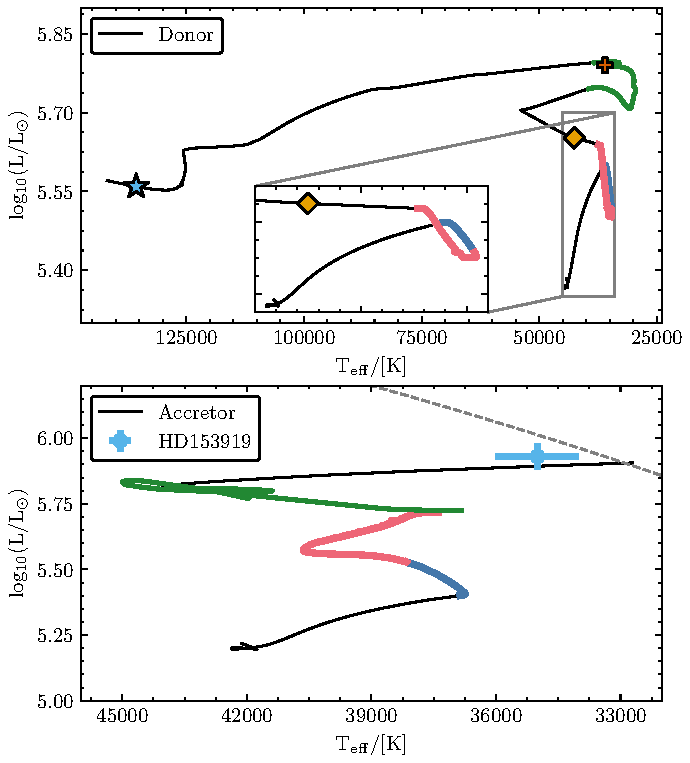
\includegraphics[width=0.5\textwidth]{xrb_fiducial_hr.pdf}
    \caption{\red{TBA}}
    \label{fig:xrb_fiducial_hr}
\end{figure}

\subsection{What do we get wrong?}

\red{Although our MESA models and monte carlo simulations provide an evolutionary pathway for the XRB, there are a few limitations that we have not addressed yet (TBD). While are accretor model reasonably matches the properties of the visible star HD153919, such as its mass, surface temperature and luminosity, we underestimate its remaining MS lifetime. the XRB has a kinematic age of $2.2\rm Myr$, with the visible star still on the MS, while our accretor model only has $0.7\rm Myr$ left on the MS after the death of the donor star, and only $0.5\rm Myr$ to reach the current radius of HD153919. There could be a couple of potential explanations for addressing this discrepancy.}

\red{
\begin{enumerate}
    \item The measured systemic velocity is lower than what it was in the past. This could happen if the XRB slows down to its current systemic velocity as it escapes the cluster potential. A higher systemic velocity in the past would imply a smaller kinematic age.
    \item A larger initial donor mass (currently assumed to be $40\,\Mdot$) would imply a shorter lifetime for the progenitor of the compact object, thereby extending time spent in the post--RLOF phase for our accretor model. This is complicated by the fact that a larger donor mass would also imply a slightly larger pre--SN mass that may be harder to explode and form a $2.5\,\Mdot$ compact object.
    \item A smaller initial accretor mass (currently assumed to be $33.5\,\Mdot$) would imply a smaller mass for the star post--RLOF, thereby extending its MS lifetime. This could be in tension with the measured luminosity of the star, as we find that (initially) lower mass accretors are less luminous at present day than what is inferred from observations.
    \item The effects of rejuvenation in the accretor are larger than currently modeled in our binaries. Rejuvenation increases the core mass, and the extra supply of fuel can extend the MS lifetime. Thus, more rejuvenation could help address the discrepancy between the MS lifetimes in our models and the XRB's kinematic age.
\end{enumerate}
}
\red{It could also be that the discrepancy could be addressed by a combination of the above factors, or something else entirely. Previous studies have also seen a 2x discrepancy in the ages as measured from single star evolutionary grids and kinematic ages.}

\red{Secondly, our donor models at carbon depletion have a total mass of $13.3\,\Mdot$ and a Carbon-Oxygen core of $11.3\,\Mdot$. Population synthesis models would predict such stars to implode and form direct collapse black holes, and not successfully explode to leave behind a $2.5\,\Mdot$ compact object. However, the explodability of massive stars is still an active area of research, with 3D simulations pointing towards a more nuanced picture than simple prescriptions just based on the core mass.} 

\subsection{Why do we need a natal kick?}

\red{Compact object that are formed in a successful supernova explosion may receive a natal kick at birth due to asymmetries in the explosion or in neutrino emission. Observationally, the natal kicks received by neutron stars is well described by a maxwellian distribution with a mean of 265km/s. However, for black holes, the story is a bit more complicated with evidence pointing towards weak or no kicks in some cases or strong kicks in others. For our X-ray binary of interest, we know that this is a runaway system from Gaia kinematics. The runaway nature does not necessarily imply that the compact object received a natal kick, as some mass lost in a spherically symmetric can also impart a systemic velocity to the binary and also induce eccentricity in the system. This is referred to as the "Blauuw kick" and the new binary orbit (if the system did not get disrupted) always has a larger orbital period (and therefore the orbital separation) because of the mass lost in the explosion. However, a decrease in the orbital period may be possible given a natal kick in a favourable direction. Given that the XRB currently is in a very tight orbit of just 3.41 days, a Blauuw kick implies that the pre-supernova orbit must have been even tighter. This may be inconsistent with most scenarios of mass transfer through RLOF, which in general leads to a widening of the orbit. Therefore, we assume that the pre-supernova orbital period was larger than the current one, and that the shrinking of the orbit is due to a natal kick received by the compact object. Not just that, for the orbit to shrink, we find that the natal kick must be directed away from the orbital velocity of the star, as seen in (insert fig)}

\section{Why not a common envelope?}

\red{Given the short period of the XRB, it may seem appealing to invoke a common envelope formation scenario for this system. In this section, we discuss why it is difficult to form this X-ray binary through a common envelope instead of stable RLOF. To start with, the visible star in the system (and the originally less massive one) has a high mass of 40-60Msun. Since this star likely did not gain any mass during a supposed common envelope phase, the original donor that formed the compact object must have been more massive than 40-60 Msun. In a common envelope phase, the donor would lose its envelope, and leave behind a core that would be far too massive to successfully explode and form a 2.5Msun compact object (however see Burrows et al etc papers). To add to that, our monte carlo experiments imply that the pre-SN donor mass is less than 15Msun, which is far too small of a core for a star that is more massive than 40-60Msun. Also, common envelope phases usually are though to occur for asymmetric binaries, and this may imply that the donor should have been much more massive than the current visible star. All of these constraints may imply that forming this X-ray binary through a common envelope phase is unlikely, and that the likely scenario may involve stable mass transfer through RLOF.}

\section{Why not Case B mass transfer?}

\red{Previous studies of this system have suggested formation pathways wherein mass transfer occurs after the donor star has left the main sequence (Case B). However, this is unlikely because of the short orbital period of the binary today. Renzo 2019 (insert citation) showed that for Case B mass transfer, the orbital period of the binary widens significantly in most cases, except for scenarios where mass transfer is non conservative ($\beta < 0.6$) \textit{and} there are extreme losses in angular momentum ($\gamma_{\rm RLOF} \geq 2$). To add to that, as Case B occurs after the donor has left the MS, the initial orbital period of the binay must have been $>10$ days, and this would have most likely increased post--MT. As we find in our monte carlo results, even with a favourable kick in the right direction, it is likely extremely rare to get the period post--SN to less than 4 days starting from a $>10$ day period pre--SN.}

\section{GW190814}

GW190814 was an exceptional event that consisted of a merger between a 23Msun black hole and 2.5Msun compact object. The GW data alone was not enough to characterize the black hole or neutron star nature of the less massive compact object, and the formation of such a system of such an asymmetric mass ratio has been puzzling for standard formation channels. 

\subsection{MESA model - GW190814}

\red{
\begin{enumerate}
    \item Based on "success" of XRB model, propose similar solution for GW190814
    \item What will be different here? - Why is XRB a TZO - kick strength and direction
    \item Why switch to lower masses - weaker winds
    \item No observational constraints other than masses - more freedom
    \item Describe fiducial GW model at Z/10 - key phases, HR diagram, final masses, donor explosion.
    \item Describe possible futures
    \item Evolve accretor as single star - next interaction depends on post-SN orbit. At smaller radii / lack of convective envelope / before RSG phase, binding energy high, merger likely. At larger radii, core envelope distincition, lower binding energy, CE ejection likely.
    \item End state - large BH (implosion) + NS/low mass BH (after successful explosion + strong kick) - asymmetric mass ratio GW event
\end{enumerate}
}

A key difference for stars at lower metallicity is that the wind mass loss becomes signifcantly weaker. From our previous MESA models at solar metallicity, we saw that the mass loss during the "WR phase" (core--helium burning) is extremely important in getting the donor star's mass down to what we expect from our monte carlo simulations. Utilizing the same stellar masses and computing their binary evolution at lower metallicity would leave us with pre-SN donor stars with sufficiently high masses that would likely fail to explode. This motivates us to lower the initial masses of our stars while trying to model the progentior of a GW190814--like system at lower metallicity. For our fiducial GW190814--like model, we start with a binary of $30\,\Mdot+25\,\Mdot$ in a 3 day orbit. We show the evolution of this binary on the HR diagram in Fig. \ref{fig:gw_hr}. Qualitatively, it follows a similar pathway as our fiducial XRB model. As stars at lower metallicity are more compact, mass transfer begins slightly later in the evolution. After $5.1 \rm Myr$, the donor star overflows its roche lobe during the MS, initiating Case A mass transfer. This phase lasts around $1 \rm Myr$, after which the donor has reached TAMS and starts contracting, detaching itself from its RL. At this stage, the donor star has a mass of $19\,\Mdot$, while the accretor has grown to about $36\Mdot$. Due to the short orbital period, tidal effects keep the accretor below critical rotation, and mass transfer remains close to fully conservative. The donor soon re--expands once it starts hydrogen shell burning, and starts a second phase of Case AB mass transfer, similar to our fiducial XRB model. At the end of this phase, we are left with a a binary of $16.5\Mdot+38.3\Mdot$ in a tight $3.85d$ orbit. Around the same time, the donor contracts and ignites helium burning in its core, and the star has a mass of $14.4\Mdot$ at helium depletion, with a carbon-oxygen core mass of $12.3\Mdot$, and a $\rm C/O$ ratio of $0.36$, which is roughly similar to what we got for our fiducial XRB. On the other hand, the accretor, which is now the more massive star in this system has a mass of $38.5\Mdot$. Assuming that the donor star successfully explodes and leaves behind a NS or a low mass BH similar to $2.5\,\Mdot$, and the strength and direction of the natal kick, we can have a variety of outcomes. Large enough kicks can potentially disrupt the binary itself, while low kicks would just slightly widen the orbit. The now more massive star will continue growing as its burns hydrogen in its core, and begin a phase of reverse MT if it overflows its RL. The outcome of a phase of reverse RLOF onto a compact object sensitively depends on the evolutionary state of the star at that point. Due to the highly assymetric mass ratio, MT is likely going to be unstable and a CE phase is likely. If the star interacts while it is still on or just past its MS, its envelope binding energies are likely going to be sufficeintly high that it would meet the same fate as out fiducial XRB and form a transient/TZO. However, if the natal kick to the first born CO is large enough but not leading to disruption, the binary can be pushed into a wide orbit where the reverse MT starts much later in the evolution of the star. This is crucial for the successful ejection of a CE, as donor stars with large and loosely bound convective envelopes are easier to eject. The star will likely develop a loosely bound convective envelope once it has expanded sufficeintly and become cool enough to be a RSG. Interaction during the RSG phase significantly increases the possibility of a successful CE ejection, and we would be left behind with a tight binary, consisting of a helium core of about $20\Mdot$ and a $2.5\Mdot$ CO. Such a massive helium core is expected to implode and form a $20\Mdot$ BH without a natal kick. We are now left with a DCO system consisting of a $20\Mdot$ BH and a $2.5\Mdot$ CO, which would then merge after a GW driven inspiral. Such a system would appear to be similar in compact object masses to GW190814. 

\begin{figure}[htbp]
    \centering
    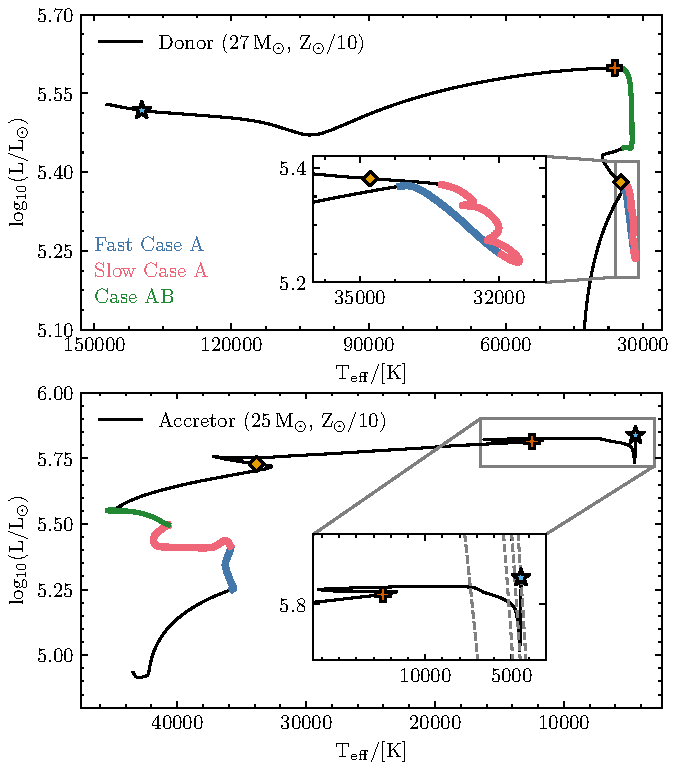
\includegraphics[width=0.5\textwidth]{gw_fiducial_hr.pdf}
    \caption{\red{TBA}}
    \label{fig:gw_hr}
\end{figure}

\section{Future evolution}

\begin{figure}[htbp]
    \centering
    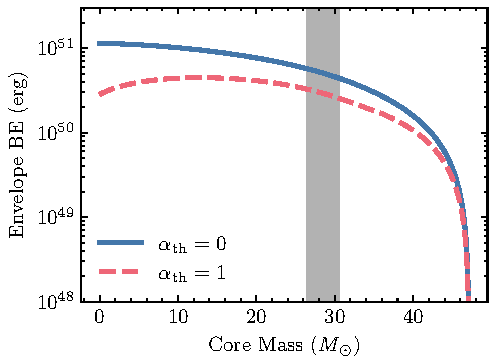
\includegraphics[width=0.5\textwidth]{xrb_be.pdf}
    \caption{\red{TBA}}
    \label{fig:xrb_be}
\end{figure}

\begin{figure}[htbp]
    \centering
    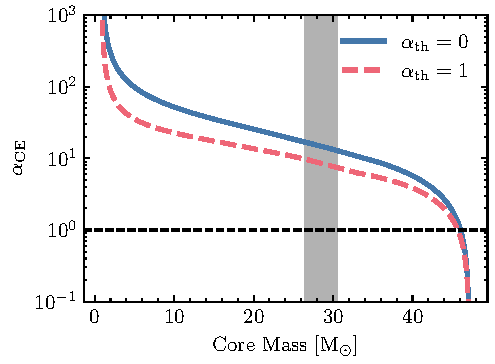
\includegraphics[width=0.5\textwidth]{xrb_alpha_ce.pdf}
    \caption{\red{TBA}}
    \label{fig:xrb_alpha_ce}
\end{figure}

Now that we have been able to chart a reasonable past evolutionary history of the XRB using our MESA binary models, we evolve the system further to see what the future of this system could look like? The current mass of the compact object is 2.5Msun while the companion is 40-60Msun that is yet to fill its roche lobe. As the star evolves further, it will grow in size and soon overflow its roche lobe. However, given the highly asymmetric nature of the system, the subsequent mass transfer is likely to soon become unstable and the compact object will plunge into the companion star's envelope, starting a phase of common envelope evolution. This phase is highly complex and multidimensional with various physical processes occuring at different time and length scales. Importantly, the success or failure of the common envelope phase is an active area of research with no concrete predictions. However, various techniques have been introduced to simulate (or skip over) this phase, enabling predictions to be made albeit at the cost of accuracy. One of the most commonly used approaches is the energy balance formalism or $\alpha \lambda$ mechanism. This parameterized method quantifies what fraction ($\alpha$) of the orbital energy is required to unbind the donor star's envelope, which is parametrized by $\lambda$. To simulate the outcome of our XRB, we evolve it till it overflows its roche lobe and the mass transfer becomes unstable (quantified by Mdot > 0.1Msun/yr). Using the orbital separation, we know how much orbital energy is available, and using the interior structure of the star, we can compute the binding energy of the envelope as well. This requires us to assume a particular definition of core, and everything above it would be considered the envelope. If a common envelope ejection is successful, what remains of the donor star is its core, and we assume that it may have some sort of response that can expand its size by up to twice that of what the core size originally was at the star of the common envelope phase. If we assume a perfect use of orbital energy to unbind the envelope, i.e $\alpha=1$, we can compute what would be the final separation between the compact object and the remnant core. If the remnant core fits inside the roche lobe of its new orbit, it implies that common envelope ejection was successful and we are left with a tight but detached binary. However, if the remnant core is too large for its final orbit, it means that there was a merger between the compact object and remnant core, and common envelope ejection was not successful. 

In Fig. \ref{fig:xrb_be}, we show the envelope binding energy of our fiducial accretor model at its current radius of about $25R_{\odot}$. We define it as 

\begin{equation}
    \rm BE(m) = \int_m^M dm' \left(-\frac{Gm'}{r(m')} + \alpha_{\rm th}u(m')\right)
\end{equation}

where $\alpha_{\rm th}$ is the parameter controlling the fraction of internal energy. Since there is no one definition for what is considered as the core, and what is the stellar envelope (especially for a MS star), we calculate the binding energy as a function of core mass. The binding energy at mass coordinate $m$ is the energy required required to lift up and eject all the stellar material above that mass coordinate. For a MS star, we consider two physically motivated definitions for the location of the core. One is the mass of the convective core, and the other is mass of the convective core \textit{and} the overlying overshooting region. These two limits span the shaded area in Fig. \ref{fig:xrb_be}. The red dashed and blue solid lines denote the binding energy curves with and without the contribution of the internal energy. Addition of internal energy provides an extra energy source which makes it easier to unbind the envelope (lower binding energy). We find that for our stellar model at its current evolutionary state, the binding energies lie between $[2.5-5.7] \times 10^{50} \rm erg$, depending on the assumed core mass definition and whether we include the internal energy or not. 

In an ensuing phase of MT, if it turns unstable, the compact object plunges into the stellar envelope and the system enters a common envelope phase. The success (successful envelope ejection leaving behind a tight binary) or failure (pfailed ejection and premature merger) is a complex hydrodynamical process that can only be approximated in 1D stellar models. This is often done with the $\alpha \lambda$ prescription, where $\lambda$ quantifies the envelope binding energy, and $\alpha$ quantifies how much of the orbital energy can be used to unbind the envelope. 

We calculate the $\alpha_{\rm CE}$ as

\begin{equation}
    \alpha_{\rm CE} \def \alpha_{\rm CE}(m) = \frac{\rm BE(m)}{-\frac{\rm GM_1 M_2}{2a_{\rm pre-CE}} + \frac{\rm Gm M_2}{2r(m)}}
\end{equation}

 A $\alpha_{\rm CE}$ greater than one implies that just the orbital energy is not sufficient to eject the envelope, and additional sources of energy are required. As can be seen in the shaded region in Fig. \ref{fig:xrb_alpha_ce}, we find that successful CE ejection requires values of $\alpha_{\rm CE}$ between $13-17$ if we exclude the internal energy and $7.5-9.5$ if we include it. These numbers are quite high, and usually imply that the common envelope phase would be unsuccessful, as the core of the star and the compact object would prematurely merge before ejecting the common envelope. Such a merger could potentially give rise to an interesting transient or even the formation of a Thorne-Zytkow object (TZO). However, due to the low likelihood of successful CE ejection, the HMXB 4U1700-37/HD153919 is unlikely to form a double compact object system, and therefore unlikely to be the progenitor of a gravitational wave source.

\section{Discussion} \label{sec:highlight}

\red{
\begin{enumerate}
    \item Very asymmetric HMXB in our own galaxy - well studied observationally, lots of constraints. Helps in charting past history
    \item sibling/analogous to GW190814 - insights from galactic binaries to weird low Z GW events
    \item common origin - conservative mass transfer + q~1 massive binaries
    \item different endings - strength and direction of natal kick - XRB shrinks (seen as XRB, future TZO), GW widens (interacts during RSG, CE ejection, GW driven merger)
    \item pathway to forming asymmetric binaries starting from symemtric ones
    \item Perhaps Case A is needed, as in Case B helium core is developed and may be unable to explode
    \item need successful explosion for both XRB/GW to form NS/low mass BH, and for GW need a strong natal kick as well
\end{enumerate}
}

\section{Conclusion} \label{sec:cite}


%% Please use the acknowledgment and contribution environments. This will 
%% be anonomyized when the "anonymous" style option is used. 
\begin{acknowledgments}

\end{acknowledgments}

\begin{contribution}

\end{contribution}

%% To help institutions obtain information on the effectiveness of their 
%% telescopes the AAS Journals has created a group of keywords for telescope 
%% facilities.
%
%% Following the acknowledgments section, use the following syntax and the
%% \facility{} or \facilities{} macros to list the keywords of facilities used 
%% in the research for the paper.  Each keyword is check against the master 
%% list during copy editing.  Individual instruments can be provided in 
%% parentheses, after the keyword, but they are not verified.
\facilities{HST(STIS), Swift(XRT and UVOT), AAVSO, CTIO:1.3m, CTIO:1.5m, CXO}

%% Similar to \facility{}, there is the optional \software command to allow 
%% authors a place to specify which programs were used during the creation of 
%% the manuscript. Authors should list each code and include either a
%% citation or url to the code inside ()s when available.
\software{astropy \citep{2013A&A...558A..33A,2018AJ....156..123A,2022ApJ...935..167A},  
          Cloudy \citep{2013RMxAA..49..137F}, 
          Source Extractor \citep{1996A&AS..117..393B}
          }

%% Appendix material should be preceded with a single \appendix command.
%% There should be a \section command for each appendix. Mark appendix
%% subsections with the same markup you use in the main body of the paper.
%%
%% Each Appendix (indicated with \section) will be lettered A, B, C, etc.
%% The equation counter will reset when it encounters the \appendix
%% command and will number appendix equations (A1), (A2), etc. The
%% Figure and Table counter will not reset.

\appendix

%% For this sample we use BibTeX plus aasjournalv7.bst to generate the
%% the bibliography. The sample7.bib file was populated from ADS. To
%% get the citations to show in the compiled file do the following:
%%
%% pdflatex sample7.tex
%% bibtext sample7
%% pdflatex sample7.tex
%% pdflatex sample7.tex

\bibliography{xrb_gw}{}
\bibliographystyle{aasjournalv7}

%% This command is needed to show the entire author+affiliation list when
%% the collaboration and author truncation commands are used.  It has to
%% go at the end of the manuscript.
%\allauthors

%% Include this line if you are using the \added, \replaced, \deleted
%% commands to see a summary list of all changes at the end of the article.
%\listofchanges

\end{document}

% End of file `sample7.tex'.
